\section{Technologien}\label{technologien}
Zum besseren Verständnis der Thematik werden in den folgenden Kapiteln verwendete Technologien erläutert. Die Grundlagen und besonderen Merkmale, der einzelnen Technologien, helfen dabei, die spätere Analyse nachvollziehen zu können. Zu den Kernsprachen, mit denen im Browser visuelle Informationen angezeigt und verändert werden können, zählen unter Anderem die Auszeichnungssprache Hyper Text Markup Language (HTML), die Gestaltungssprache Cascading Style Sheets (CSS) und die Skriptsprache JavaScript. Auf diesen Sprachen baut das SAP UI5-Framework auf. Frameworks sind in sich konsistente Bibliotheken, die gewisse Sprachkonstrukte, welche häufig in der Entwicklung benötigt werden, zur Verfügung stellen. Mit dem Einsatz eines Frameworks verfolgt man das Ziel oft geschriebenen Programm Code in eine Art \textit{Bausatz-Konstruktions-Set} auszulagern. So lässt sich ein einmal durchgeführter Entwicklungsprozess beliebig oft und mit weit weniger Aufwand bewerkstelligen, als wenn man jedes Mal den Programmcode von neuem entwickeln müsste.

\subsection{HTML5}
In diesem Kapitel wird zuerst die Entstehung des aktuellen HTML-Standards beschrieben, von den Anfängen bis zur heute gültigen Spezifikation. Außerdem werden die Ziele näher definiert sowie der allgemeine Aufbau eines HTML-Dokuments aufgezeigt. Abschließend sind die wichtigsten neuen Elemente der HTML5 Sprache ausführlich dargelegt.

\subsubsection{Historie} HTML5 ist die aktuell empfohlene Sprache des World Wide Web Consortium (W3C) und stellt eine der Kernsprachen des World Wide Web (WWW) dar. Im November 1995 erklärte das W3C HTML2.0 zum offiziellen Sprachstandard. Grundlegende Unterschiede zwischen Version 1.0 und 2.0 existieren nicht. Version 3.0 der HTML-Spezifikation ist gänzlich am Browsermarkt vorbei definiert worden. Aus diesem Grund wurde HTML3.2 ab Januar 1997 zum Nachfolger von Version 2.0 gemacht. Die folgende Entwicklung, der Spezifikation, brachte 1999 die überarbeitete Version 4.01 hervor. Im selben Zug wurde CSS, als Gestaltungssprache für HTML, immer mehr fokussiert. So begann die Fragmentierung, der HTML-Spezifikation, und es existierten drei Versionen zur selben Zeit. Nämlich HTML4.01 \textit{strict}, die dem eigentlich definiertem HTML am nächsten kam. HTML4.01 \textit{transitional}, in welcher auch einige übliche physische Textauszeichnungen vorgesehen waren. \glqq Physische Textauszeichnungen haben Bedeutungen wie \textit{fett} oder \textit{kursiv}, stellen also direkte Angaben zur gewünschten Schriftformatierung dar. Bei physischen Elementen sollte der Web-Browser eine Möglichkeit finden, den so ausgezeichneten Text entsprechend darzustellen.\grqq{}\cite{SelfHTML20141}. Sie wurde als Übergangslösung entwickelt. Die dritte Variante ist HTML4.01 \textit{frameset}. Der einzige Unterschied zur \textit{transitional} Variante ist, dass sich im Rumpf eines HTML-Dokuments ein Element verändert. Neben HTML wurde ab Januar 2000 auch eine Extensible HTML (XHTML) genannte Spezifikation entwickelt, die HTML mit dem Extensible Markup Language (XML) Standard vereinen sollte. XHTML ist allerdings nicht als eigenständige Sprache zu verstehen, sondern als eine Serialisierungsform für HTML unter Verwendung von XML. Mit HTML5 wurde die Spezifikation nicht mehr durch die SGML - eine Metasprache zur Definition von Auszeichnungssprachen - sondern durch ein \textit{Document Objekt Model} (DOM) beschrieben. Die in dieser Version neu eingeführten Elemente sollten es erlauben HTML-Dokumente semantisch klarer zu strukturieren.(vgl. \cite[S.20ff]{MunzHTML2012}) Im Oktober 2014 wurde HTML5 vom W3C zum De-facto Standard des WWW erklärt. Heute existiert neben der Spezifikation des W3C auch noch ein sogenannter \glqq lebender Standard\grqq{} der \textit{Web Hypertext Application Technology Working Grou}p (WHATWG). Die WHATWG ist ein Zusammenschluss von Unternehmen, wie zum Beispiel Mozilla Foundation, Opera Software und Apple. Der allgemeine Sprachgebrauch von HTML ist dadurch nicht an die W3C Spezifikation gebunden. Er erstreckt sich über den \textit{lebenden Standard} der WHATWG hinaus und beinhaltet zahlreiche Schnittstellen zu anderen Technologien. Abbildung \ref{fig:html5specs} verdeutlicht diese Situation.
	
\vspace{1em}
\begin{figure}[htb]
  \centering
  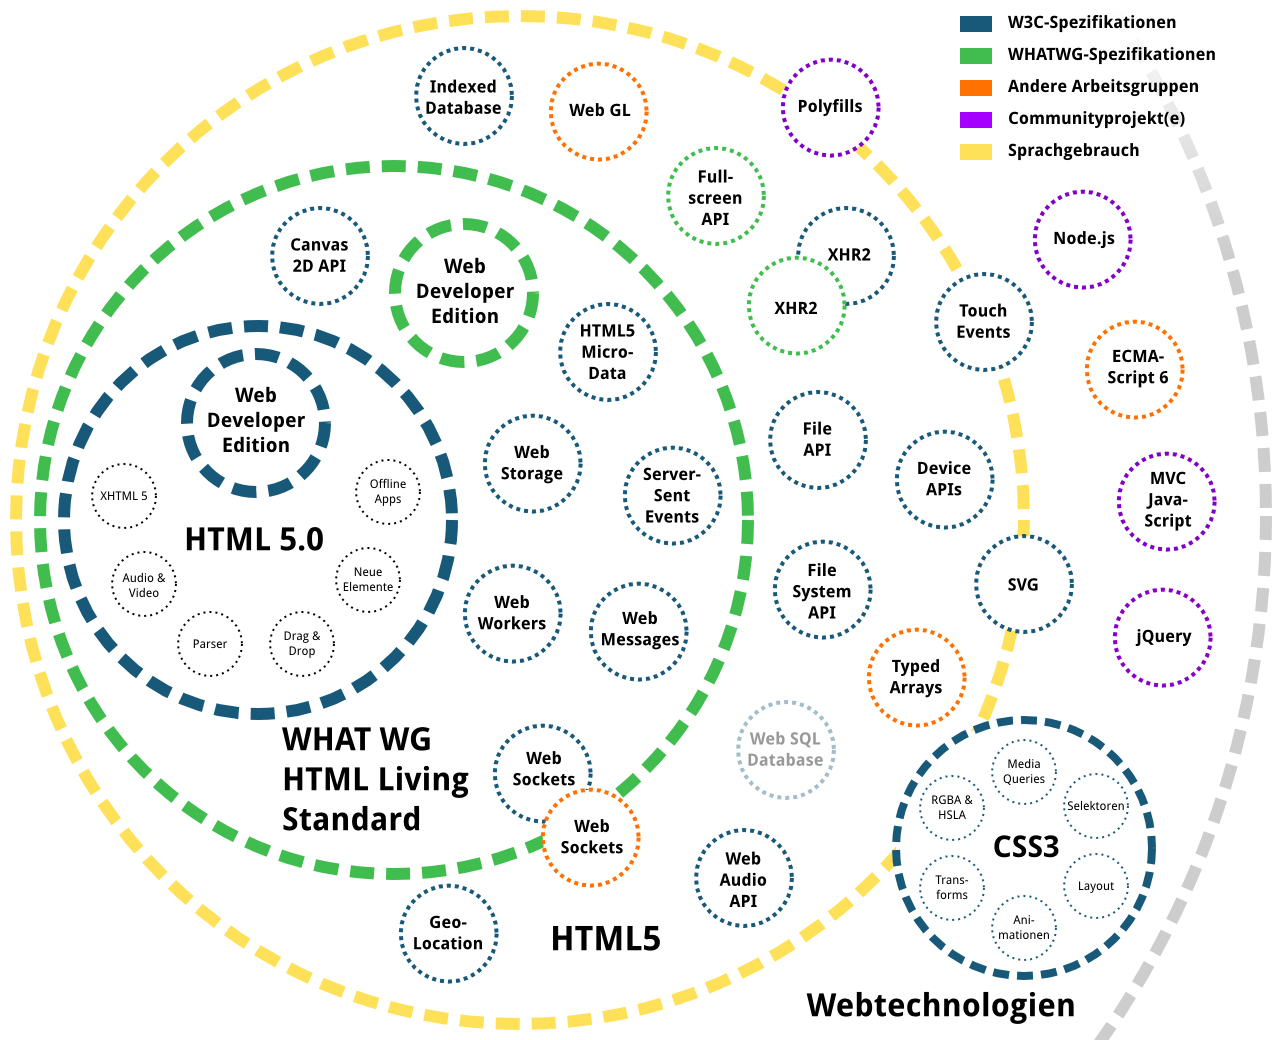
\includegraphics[width=0.75\linewidth]{abb/html5_specs}
  \caption[HTML5 Spezifikationen Übersicht]{HTML5 Spezifikationen Übersicht \cite{PeteKroe2014}}
  \label{fig:html5specs}
\end{figure}

\subsubsection{Ziele} HTML5 wurde mit besonderem Augenmerk auf die Kompatibilität entwickelt. Vorhandene Spezifikationen wie HTML4.01, XHTML1.0 und DOM2 sollten unter einem Dach gebündelt werden. Hierdurch wird der vorangegangenen Fragmentierung entgegen gewirkt. Bereits vorhandene Inhalte müssen weitestgehend unterstützt werden, auch wenn sie nicht zur HTML5-Spezifikation gehören. Beispielsweise werden fehlerhaft verschachtelte Elemente trotzdem akzeptiert. \textit{Graceful degradation} ist als ein weiteres Ziel für HTML5 definiert worden und bedeutet soviel wie \textit{Schrittweise Abstufung}. Es stellt sicher, dass ein HTML-Dokument auch dann verarbeitet wird wenn der verwendete Browser ein bestimmtes benutztes Element nicht unterstützt. Weiter galt für die Spezifikation, dass schon vorhandene Techniken, die weitläufig verbreitet sind, nicht neu entwickelt werden sollten. Stattdessen sollten sie übernommen werden. Dies beruht auf dem Umstand, dass die Browserhersteller jeweils ihre eigenen Techniken bevorzugen, weiter entwickeln und dadurch auch für ihre Verbreitung sorgen. Evolution statt Revolution war der Vorsatz für HTML5. (X)HTML wurde weiterentwickelt und nicht von Grund auf neu definiert. In Tabelle \ref{tab:html5browserkomp} ist die, zum aktuellen Zeitpunkt, verfügbare Unterstützung von HTML5 in den gängigsten Browsern abzulesen.

\vspace{1em}
\begin{center}
  \begin{tabular}{ | l | l | c | }
  \hline
  \textbf{Hersteller} & \textbf{Desktop/Mobile} & \textbf{Version} \\ \hline \hline
  Mozilla & Firefox & 4.0\\
	\hline
	& Firefox Mobile & 16\\
	\hline
	Google & Chrome & 10\\
	\hline
	& Chrome Mobile & 25\\
	\hline
	& Android & 4.0\\
	\hline
	Apple & Safari & 5.1\\
	\hline
	& Safari iOS & 5.1\\
	\hline
	Microsoft & Internet Explorer & 10\\
	\hline
	& Windows Phone & 8\\
	\hline
	Opera Software & Opera & 11.64\\
	\hline
	Blackberry & Browser & 10\\
  \hline
  \end{tabular}
\captionof{table}{HTML5 Browserkompatibilität}
\label{tab:html5browserkomp}
\end{center}

\subsubsection{Aufbau} Jedes HTML-Dokument beginnt mit dem sogenannten \texttt{doctype}. Dieser legt fest, mit welcher Syntax das Dokument aufgebaut ist und wie das Dokument vom Browser verarbeitet werden soll. Verschiedene Varianten wie \textit{strict}, \textit{transitional} und \textit{frameset} sind in HTML5 nicht vorgesehen. In den Vorgängerversionen musste die Variante jedoch mit angegeben werden, um eine eindeutige Interpretation des Dokumententypen zu gewährleisten. Listing \ref{lst:html401doctype} zeigt die beiden \texttt{doctypes} von HTML4.01 und XHTML1.0. Durch die Abwärtskompatibilität von HTML5 sind auch diese \texttt{doctypes} heute noch gültig und das Dokument wird korrekt vom Parser interpretiert werden.

\vspace{1em}
\begin{lstlisting}[language=HTML5, caption=(X)HTML4.01 \texttt{doctype}-Element, label=lst:html401doctype]
<!DOCTYPE HTML PUBLIC "-//W3C//DTD HTML4.01//EN"
  "http://www.w3.org/TR/html4/strict.dtd">
<!DOCTYPE HTML PUBLIC "-//W3C//DTD HTML4.01 Transitional//EN"
  "http://www.w3.org/TR/html4/loose.dtd">
<!DOCTYPE HTML PUBLIC "-//W3C//DTD HTML4.01 Frameset//EN"
  "http://www.w3.org/TR/html4/frameset.dtd">
<!DOCTYPE html PUBLIC "-//W3C//DTD XHTML 1.0 Strict//EN"
  "http://www.w3.org/TR/xhtml1/DTD/xhtml1-strict.dtd">
\end{lstlisting}
	
Listing \ref{lst:html5doctype}	hingegen zeigt das \texttt{doctype} von HTML5. Es wurde stark gekürzt, im Vergleich zum \texttt{doctype} von HTML4.01 und XHTML1.0. Groß- und Kleinschreibung ist nicht von Bedeutung innerhalb des \texttt{doctype}. 

\vspace{1em}
\begin{lstlisting}[language=HTML5, caption=HTML5 \texttt{doctype}-Element, label=lst:html5doctype]
<!DOCTYPE html>
\end{lstlisting}		
	
Nach dem \texttt{doctype} folgt der weitere Aufbau des Dokuments in HTML-Syntax. Diese teilt sich auf in Elemente und Attribute, die diesen Elementen zugeordnet und mit Werten versehen werden können. Für die meisten Elemente existieren Start- und Endmarkierungen. Für einige Elemente sind die Start- bzw. Endmarkierungen optional, für andere wiederum verpflichtend, in die Dokumentstruktur zu setzen. In Listing \ref{lst:html5basicdoc} sieht man ein valides HTML5 Dokument mit den Grund Elementen für eine komplett leere Seite.(vgl. \cite[S.58]{KronHTML2011})

\vspace{1em}
\begin{lstlisting}[language=HTML5, caption=HTML5 Basis Dokument, label=lst:html5basicdoc]
<!DOCTYPE html>
<html>
 <head>
   <title>Beispieltitel</title>
 </head>
 <body>
   <h1>Ueberschrift 1</h1>
 </body>
</html>
\end{lstlisting}
	
\subsubsection{Wichtige neue Sprachelemente} In HTML5 wurden die Mikrodaten mit aufgenommen. Mikrodaten bieten eine weitere Möglichkeit das HTML-Dokument semantisch zu spezifizieren. Metadaten, wie z.B. der verwendete Zeichensatz, lassen sich so festlegen. Browser und Webseiten können über die Mikrodaten-API gesetzte Werte auslesen und weiter verarbeiten. Auch Suchmaschinen können auf die Metadaten zugreifen, verwenden sie jedoch heutzutage weitestgehend nicht mehr. Aus diesem Grund tragen die Metadaten zwar zur semantischen Struktur des HTML bei, können aber aus Sicht der Suchmaschinenoptimierung getrost vernachlässigt werden.(vgl. \cite{SelfHtml20142}) Weiter kann man bei Mikrodaten davon sprechen, \glqq [...] dass sie auf Name/Werte-Paaren basieren. Jedes Mikrodatenvokabular definiert eine Menge benannter Eigenschaften.\grqq{}\cite[S.174]{PilgDurc2011} Listing \ref{lst:html5meta} zeigt beispielhaft das \texttt{head}-Element eines HTML-Dokuments mit vier eingeschlossenen \texttt{meta}-Elementen. Unter anderem wird mit dem ersten \texttt{meta}-Element der Zeichensatz näher definiert. Das \texttt{meta}-Element mit Namen \texttt{viewport} dient dazu, die Skalierung auf Mobilgeräten zu unterdrücken, damit die Seite sich an den \texttt{viewport} anpasst.

\vspace{1em}
\begin{lstlisting}[language=HTML5, caption=HTML5 \texttt{meta}-Element, label=lst:html5meta]
<head>
  <meta charset="utf-8">
  <meta name="viewport" content="width=device-width;" />
  <meta name="keywords" content="Lorem ipsum">
  <meta name="author"   content="dolor sem it">
</head>
\end{lstlisting}
		
Zwei weitere neue Elemente in HTML5 sind das \texttt{header}- und \texttt{footer}-Element. Üblich ist es im \texttt{header}-Element einer Website Komponenten wie das Logo, das Menü und den Titel unterzubringen. Im \texttt{footer}-Element hingegen werden Kontakt, Impressum und das Copyright aufgeführt. In Listing \ref{lst:html5header} ist die Platzierung des \texttt{header}- und \texttt{footer}-Elements innerhalb eines \texttt{body}-Elements zu sehen.

\vspace{1em}
\begin{lstlisting}[language=HTML5, caption=HTML5 \texttt{header}- und \texttt{footer}-Element, label=lst:html5header]
<body>
  <header>
    <img src="logo.gif" alt="logo">
    <h1>Ueberschrift</h1>
  </header>
  <footer>
     <a href="kontakt.html">Kontakt</a>
  </footer>
</body>
\end{lstlisting}
	
Um ein HTML-Dokument nach heutigen Maßstäben korrekt zu strukturieren, wurden einige Elemente der Spezifikation hinzugefügt. So lässt sich die Navigation nun mit dem \texttt{nav}-Element umschließen, wie in Listing \ref{lst:html5struct} ab Zeile 3 zu sehen. \glqq Das \texttt{section}-Element repräsentiert einen allgemeinen Abschnitt in einem Dokument oder einer Anwendung. Ein Abschnitt ist in diesem Kontext eine thematische Gruppierung von Inhalten, die üblicherweise unter einer Überschrift stehen. Beispiele für Abschnitte wären Kapitel, die verschiedene Tabs in einem Dialog mit Tabs oder die nummerierten Abschnitte einer wissenschaftlichen Arbeit.[...] Das \texttt{article}-Element repräsentiert eine abgeschlossene Einheit in einem Dokument, einer Anwendung oder einer Site, die unabhängig verbreitet oder wiederverwendet werden kann, z.B. in RSS-Feeds. Es könnte beispielsweise ein Forenbeitrag, ein Zeitschriften- oder Zeitungsartikel, ein Blog-Eintrag, ein Benutzerkommentar, ein interaktives Widget oder Gadget oder ein Element mit unabhängigem Inhalt enthalten.

\vspace{1em}
\begin{lstlisting}[language=HTML5, caption=HTML5 Struktur Elemente, label=lst:html5struct]
<body>
  <header>
    <nav>
      <ul>
        <li><a href="#link_1.html">Link</a></li>
        ...
      </ul>
    </nav>
  </header>
  <main>
  <article>
    <h1>Ueberschrift</h1>
    <p>Dies ist eine Beispiel HTML5-Seite</p>
  </article>
  <aside>
    <section>
      <h2>Ueberschrift</h2>
      <ul>
        <li><a href="link_1.html">Link</a></li>
        ...
      </ul>
    </section>
  </aside>
  </main>
  <footer>
  </footer>
</body>
\end{lstlisting}
	
Das \texttt{aside}-Element repräsentiert einen Abschnitt einer Seite, der Inhalte enthält, die sich zwar auf den das \texttt{aside}-Element umgebenden eigentlichen Inhalt der Seite beziehen, aber als von ihm unabhängig betrachtet werden können. In Druckwerken werden derartige Abschnitte häufig als Seitenleisten dargestellt. Das Element kann für typografische Effekte wie herausgehobene Zitate oder Seitenleisten, für Werbung, für Gruppen von \texttt{nav}-Elementen und andere Inhalte verwendet werden, die als vom eigentlichen Inhalt der Seite getrennt betrachtet werden können.\grqq{}\cite[S.43]{PilgDurc2011} Das neue \texttt{main}-Element ist zur Auszeichnung des Seitenhauptinhalts vorgesehen. Mit dieser Auszeichnung lässt sich z.B. mit Screenreadern direkt zum Hauptinhalt springen. Alle genannten Elemente sind in Listing \ref{lst:html5struct} in ihrer vorgesehenen Reihenfolge abgebildet. \glqq Damit auch ältere Internet Explorer der Versionen 6-8 die neuen HTML5-Elemente darstellen können, kann ein kurzes JavaScript eingebunden werden. Am einfachsten ist es, dieses nicht auf dem eigenen Server vor zuhalten, sondern direkt von Google abzurufen. Dies hat überdies den Vorteil, dass es oft schon im Browser-Cache der Nutzer vorhanden ist. Der Aufruf erfolgt in einem \textit{Conditional Comment}, der nur vom Internet Explorer (IE) kleiner als Version 9 (lt IE 9) verstanden wird. Alle andere Browser ignorieren dies als reinen Kommentar.\grqq{}\cite{SelfHtml20143} In Listing \ref{lst:html5fallback}	 ist der beschriebene Rückfallmechanismus verdeutlicht.

\vspace{1em}
\begin{lstlisting}[language=HTML5, caption=HTML5 Internet Explorer Fallback, label=lst:html5fallback]
<head>
  <meta charset="utf-8">
  <!--[if lt IE 9]>
  <script src="http://goo.gl/RfQF7"></script>
  <![endif]-->
  <title>HTML5-Seite mit Grundstruktur</title>
</head>
\end{lstlisting}
	
Eingabefelder sind in den meisten Applikationen unabdingbar. Aus diesem Grund wurden in HTML5 eine Vielzahl an \texttt{input}-Elementen hinzugefügt. So müssen keine komplizierten Workarounds mit JavaScript oder anderen Skriptsprachen mehr verwendet werden. \glqq Das typische HTML5-Formular unterscheidet sich nicht fundamental von seinen in HTML4.01 oder XHTML1 geschriebenen Gegenstücken. Alle alten Formularelemente sind noch da und verhalten sich weitgehend wie bisher. Die Neuerungen bestehen aus einigen neuen Funktionen, Attributen und APIs und aus einer ganzen Reihe neuer möglicher Werte für das \texttt{type}-Attribut des \texttt{input}-Elements.\grqq{}\cite[S.176]{KronHTML2011} In Listing \ref{lst:html5input} sind beispielhaft einige neue Werte des \texttt{type}-Attributs ausgeführt. Eingabefelder des Typs \texttt{tel, email} oder \texttt{url} sind vom Verständnis her simple Texteingabefelder. Als wichtige Besonderheit lässt sich bei \texttt{email}- und \texttt{url}-Feldern aber ihre eingebaute Validierung nennen. Verwendet man die Validierung werden nur gültige URLs bzw. E-Mails zugelassen. Für ein \texttt{tel}-Feld gilt dies nicht. Außerdem wird auf Smartphones und Tablet-Geräten die angezeigte Bildschirmtastatur entsprechend des erwarteten Eingabetyps für eine optimale Eingabe angepasst dargestellt.(vgl. \cite[S.178]{KronHTML2011}) So wird bei einer erwarteten E-Mail Adresse das \texttt{@}-Symbol direkt auf der Bildschirmtastatur als eigene Taste mit angezeigt, was normalerweise nicht der Fall ist. Einige der neuen Elementausprägungen besitzen noch zusätzliche Attribute, die die Eingabemöglichkeit weiter einschränken und präzisieren können. Zu sehen in Zeile 5 von Listing \ref{lst:html5input} im \texttt{time}-Feld, bei dem die erwartete Zeit nur von 9:00 Uhr bis 17:00 Uhr einstellbar ist. \texttt{input}-Elemente können, über das \texttt{required}-Attribut, außerdem als Pflichtfeld markiert werden.

\vspace{1em}
\begin{lstlisting}[language=HTML5, caption=HTML5 \texttt{input}-Element, label=lst:html5input]
<body>
  <input type="tel">
  <input type="email">
  <input type="url">
  <input type="time" min="09:00" max="17:00">
  <input type="date" required="required">
</body>
\end{lstlisting}
	
Für multimediale Inhalte auf Webseiten wurden der Spezifikation passende Elemente hinzugefügt. Das \texttt{canvas}-Element \glqq [...] stellt eine Fläche zur Verfügung, auf die mittels JavaScript dynamische Bitmap-Grafiken gezeichnet werden können. So lassen sich Animationen erstellen, Diagramme zeichnen, eigene Interface-Elemente kreieren und Videos manipulieren\grqq{}\cite[S.353]{KronHTML2011} Für Audio- und Videoinhalte wurden gleichnamige Elemente geschaffen. 
	
\subsection{CSS3}
Das Kapitel CSS3 erläutert kurz die Notwendigkeit von CSS und geht dann weiter auf die Einbindung in einem HTML-Dokument ein. Anschließend wird die Syntax der Gestaltungssprache beschrieben. Einige Eigenheiten wie Selektoren und Pseudoklassen werden erklärt, um dann zum Box-Modell zu kommen. Abgerundet wird das Kapitel mit der Definition der spezifischen Stylesheets, die gerade in der Web-Entwicklung ihre Stärken zeigen.

\subsubsection{Einleitung}
\glqq Cascading Style Sheets [...] bieten mächtige Möglichkeiten, die Präsentation eines Dokuments oder einer Sammlung von Dokumenten zu beeinflussen. Offensichtlich ist CSS ohne irgendein Dokument ziemlich nutzlos, da es keine Inhalte zu präsentieren gäbe.\grqq{}\cite[S.1]{MeyeCasc2005} CSS gehört zu den Kernsprachen des WWW. \glqq Zuallererst ermöglicht CSS eine wesentlich umfangreichere Gestaltung des Aussehens eines Dokuments, als HTML das jemals konnte, nicht einmal als die Präsentationselemente einen Großteil der Sprache ausmachten. Mit CSS kann für jedes Element eine eigene Text- und Hintergrundfarbe festgelegt werden. Jedes Element lässt sich zudem mit einem Rahmen versehen; der Platz um ein Element herum kann in der Größe verändert werden und es kann Einfluss auf die Groß- und Kleinschreibung genommen werden. Mit CSS können Sie außerdem bestimmen, wie fett bestimmte Textteile dargestellt werden sollen, welche Dekoration (z.B. Unterstreichungen) verwendet werden soll, wie groß die Abstände zwischen einzelnen Buchstaben und Wörtern sein sollen und ob der Text überhaupt angezeigt wird.\grqq{}\cite[S.4]{MeyeCasc2005}

\subsubsection{Einbindung} Um eine Webseite überhaupt mit CSS zu gestalten, muss es innerhalb eines HTML-Dokuments eingebunden sein. Dies ist auf drei verschiedene Arten möglich. Die erste Möglichkeit ist das \texttt{link}-Element. \glqq CSS benutzt dieses Tag, um Stylesheets mit dem Dokument zu verbinden.[...] Stylesheets, die nicht im HTML-Dokument selbst enthalten sind, sondern von außen eingebunden werden, bezeichnet man als externe Stylesheets[...].Um ein Stylesheet erfolgreich zu laden, muss sich ein \texttt{link} innerhalb des \texttt{head}-Elements befinden, darf aber nicht innerhalb eines anderen Elements wie etwa \texttt{title} stehen.\grqq{}\cite[S.14]{MeyeCasc2005} In Listing \ref{lst:css3einbindunglink} ist die Einbindung eines externen Stylesheets über das \texttt{link}-Element zu sehen.
	
\vspace{1em}
\begin{lstlisting}[language=HTML5, caption=Stylesheet Einbindung über \texttt{link}-Element, label=lst:css3einbindunglink]
<head>
  <link rel="stylesheet" type="text/css" href="beispiel.css" />
</head>
\end{lstlisting}

Eine andere Möglichkeit wäre, das CSS direkt innerhalb eines \texttt{style}-Elements zu positionieren. Ein Element vom Typ \glqq \texttt{style} sollte immer zusammen mit dem Attribut \texttt{type} verwendet werden. Im Fall eines eingebetteten CSS-Dokuments ist der korrekte Wert \texttt{text/css}, genau wie bei dem Element \texttt{link}.[...] Die Stildefinition zwischen den öffnenden und schließenden \texttt{style}-Tags bezeichnet man als Dokumenten-Stylesheet oder auch als eingebettetes Stylesheet[...].\grqq{}\cite[S.19]{MeyeCasc2005} Listing \ref{lst:css3einbindungstyle} zeigt ein solches eingebettetes Stylesheet.

\vspace{1em}
\begin{lstlisting}[language=HTML5, caption=Stylesheet Einbindung über \texttt{style}-Element, label=lst:css3einbindungstyle]
<head>
	<title>Dokument mit Formatierungen</title>
	<style type="text/css">
		body { color: purple; background-color: #d8da3d; }
	</style>
</head>
\end{lstlisting}
	
Als letzte Möglichkeit kann man ein Stylesheet bzw. Style-Informationen direkt einem HTML-Element anhängen. \glqq Durch das direkte Festlegen von Formaten, umgangsprachlich auch \glqq Inline-Style\grqq{} genannt, gehen viele Vorteile verloren. Der Wartungsaufwand steigt während sich die Flexibilität verringert. Inline-Styles sind an ein Dokument gebunden und können nicht an zentraler Stelle bearbeitet werden.\grqq{}\cite{SelfHtml20144} In Listing \ref{lst:css3einbindunghtml} wird dem \texttt{span}-Element ein \glqq Inline-Style\grqq gegeben.

\vspace{1em}
\begin{lstlisting}[language=HTML5, caption=Stylesheet Einbindung in \texttt{html}-Element, label=lst:css3einbindunghtml]
<span style="font-size: small;">Text</span>
\end{lstlisting}
	
Innerhalb von CSS-Dateien kann man wiederum mit der Anweisung \texttt{@import} den Browser dazu bringen weitere Stylesheets nachzuladen und zu verwenden. Zu beachten ist, dass die \texttt{@import} Direktive vor allen anderen CSS Befehlen steht, bei den eingebetteten wie auch bei den externen Stylesheets.(vgl. \cite[S.20]{MeyeCasc2005})

\subsubsection{Syntax} Die Syntax von CSS ist denkbar einfach. Sie besteht im Wesentlichen aus dem Selektor und dem Deklarationsblock. Ein Selektor entspricht in den häufigsten Fällen dem gleichnamigen HTML-Element. Der Deklarationsblock besteht wiederum aus mindestens einer Deklaration.(vgl. \cite[S.26]{MeyeCasc2005}) \glqq Eine Deklaration besteht dabei immer aus einer Eigenschaft, die mit einem Wert durch einen Doppelpunkt verbunden ist. Abgeschlossen wird die Deklaration durch ein nachgestelltes Semikolon. Auf den Doppelpunkt und das Semikolon kann eine beliebige Anzahl von Leerzeichen (also auch keines) folgen. Fast immer besteht der Wert aus einem einzelnen Schlüsselwort oder einer durch Leerzeichen getrennten Liste aus mehreren Schlüsselwörtern, die für die genannte Eigenschaft zulässig sind.\grqq{}\cite[S.28]{MeyeCasc2005} Verwendet man in der Deklaration ungültige Eigenschaften oder Werte werden diese einfach ignoriert. Listing \ref{lst:css3syntax} zeigt die Syntax beispielhaft.

\vspace{1em}
\begin{lstlisting}[language=CSS, caption=CSS3 Syntax Beispiel, label=lst:css3syntax]
Selektor [, Selektor2, ...] {
  Eigenschaft1: Wert1;
  ...
  EigenschaftN: WertN[;]
}
\end{lstlisting}

Um sich wiederholende Designregeln zusammenfassen zu können, lassen sich Selektoren in CSS gruppieren. Dabei werden die zu gruppierenden Selektoren durch ein Komma voneinander getrennt und dann die zu gestaltenden Eigenschaften mit den entsprechenden Werten genannt, wie in Listing \ref{lst:css3group} zu sehen.

\vspace{1em}
\begin{lstlisting}[language=CSS, caption=CSS3 Gruppierung, label=lst:css3group]
h1, h2, p {
  color: black;
}
\end{lstlisting}

\subsubsection{Selektoren} CSS arbeitet wie HTML auch mit dem DOM. \glqq Der erste Vorteil, der sich aus dem Verständnis dieses Modells ergibt, ist die Möglichkeit, Selektoren für Nachfahren (auch als Kontext-Selektoren bezeichnet) zu definieren. Die Definition von Selektoren für Nachfahren besteht aus dem Festlegen von Regeln, die nur für bestimmte hierarchische Strukturen gelten.\grqq{}\cite[S.48]{MeyeCasc2005} Der erstgenannte Selektor ist das Elternelement. Mittels eines Leerzeichens wird das Nachfahrenelement vom Elternelement getrennt. In Listing \ref{lst:css3kids} wird angegeben, dass jedes \texttt{strong}-Element innerhalb eines \texttt{h1}-Elements eine besondere Formatierung erhält. Konkret bedeutet das in diesem Fall, dass die Schriftgröße 14pt und die Schriftgewichtung, welche die Dicke und Stärke festlegt, \texttt{bold} sein soll. Zu beachten ist, dass so sämtliche Nachfahren des \texttt{h1}-Elements entsprechend formatiert werden. Es gibt auch die Möglichkeit die Formatierung nur auf einen direkten Nachfahren, ein sogenanntes Kindelement, zu beschränken. Um dies zu erreichen werden Eltern- und Kindelement nicht durch ein Leerzeichen voneinander getrennt, sondern durch das Größer-als-Zeichen (\textgreater).

\vspace{1em}
\begin{lstlisting}[language=CSS, caption=CSS3 Selektoren für Nachfahren, label=lst:css3kids]
h1 strong {
  font-size:   14pt;
  font-weight: bold;
}
\end{lstlisting}

Das gleiche Verfahren kann auch auf Nachbarelemente angewandt werden. Nur wird hierbei ein anderes Kombinatorenzeichen benötigt, nämlich das Plus (+).\par \glqq Zusätzlich zu den rohen Dokument-Elementen gibt es noch zwei weitere Arten von Selektoren: Klassenselektoren und ID-Selektoren, mit denen sich Stildefinitionen unabhhängig von den Elementen eines Dokuments zuweisen lassen. Diese Selektoren können eigenständig oder zusammen mit Elementselektoren verwendet werden. Allerdings ist es hierfür notwendig, die Dokumentteile entsprechend zu markieren. Die Benutzung dieser neuen Selektoren erfordert daher [...] Voraussicht und Planung.\grqq{}\cite[S.34ff]{MeyeCasc2005} Des Weiteren muss die HTML-Auszeichnung angepasst werden sollten Klassen- und/oder ID-Selektoren verwendet werden. Konkret bedeutet dies, dass jedem HTML-Element ein \texttt{class}- und/oder \texttt{id}-Attribut hinzugefügt werden muss, sofern es von den CSS Regeln beachtet werden soll. Zu beachten ist, dass eine vergebene ID im gesamten HTML-Dokument einzigartig sein muss, wohingegen eine vergebene Klasse auf mehrere HTML-Elemente und auf ein HTML-Element auch mehrere Klassen angewandt werden können. (vgl. \cite{W3ScCss2014}) Listing \ref{lst:css3idclass} zeigt einen solchen ID-Selektor, einen Klassenselektor und einen Klassenselektor der nur bei \texttt{p}-Elementen gilt, die das \texttt{class}-Attribut besitzen.

\vspace{1em}
\begin{lstlisting}[language=CSS, caption=CSS3 Klassen- und ID-Selektoren, label=lst:css3idclass]
<div id="ID">
  <p class="Klasse"></p>
</div>

div#ID {
  text-align: center;
  color:      red;
}
.Klasse {
  text-align: center;
  color:      red;
}
p.Klasse {
  text-align: center;
  color:      red;
}
\end{lstlisting}
	
\subsubsection{Pseudoklassen} Neben den genannten Selektoren gibt es noch einen weiteren Typ von Selektoren. Die sogenannten Pseudoselektoren für die Pseudoklassen. \glqq Mit diesen Selektoren [... lassen sich] Stildefinitionen auf Strukturen zuweisen, die nicht unbedingt im Dokument vorkommen müssen, oder auch [... Pseudo]klassen, die vom Zustand bestimmter Elemente oder sogar vom Zustand des Dokuments selbst abhängen. Anders gesagt, werden die Stile, basierend auf etwas anderem als der Struktur des Dokuments, auf Teile des Dokuments angewendet.\grqq{}\cite[S.53ff]{MeyeCasc2005} Um beispielsweise einen Link in einem Dokument farblich zu markieren, sobald er besucht wurde, wäre eigentlich für jeden Zustand des Links eine eigene Klasse nötig. Diese Klasse müsste sich ständig ändern je nachdem ob der Nutzer den Link schon besucht hat oder nicht. Um diesen Umstand zu verhindern, existieren die Pseudoselektoren und Pseudoklassen. Im Fall eines \texttt{a}-Elements werden die Pseudoklassen \texttt{link} und \texttt{visited} bereitgestellt, um den Effekt zu erzeugen. Diese Klassen werden dem \texttt{a}-Element durch CSS selber hinzugefügt bzw. wird ein \texttt{a}-Element, das ein \texttt{href}-Attribut besitzt und noch nicht besucht wurde mit der Pseudoklasse \texttt{link} versehen. Die Pseudoklasse \texttt{visited} bezieht sich auf \texttt{a}-Elemente mit \texttt{href}-Attribut die schon besucht wurden. Listing \ref{lst:css3pseudo} zeigt ein solches \texttt{a}-Element und die beiden Pseudoselektoren.

\vspace{1em}
\begin{lstlisting}[language=CSS, caption=CSS3 Pseudoklassen und -selektoren, label=lst:css3pseudo]
<a href="http://www.example.com">Example.com</a>

/* unvisited link */
a:link {
  color: #FF0000;
}

/* visited link */
a:visited {
  color: #00FF00;
}
\end{lstlisting}

\subsubsection{Box-Modell} \glqq CSS geht davon aus, dass jedes Element eine oder mehrere rechteckige Boxen erzeugt, die Element-Boxen genannt werden.[...] Im Kern besitzt jede Box einen Inhaltsbereich (content area). Dieser wird umgeben von optionalen Innenabständen (padding), Rahmen (borders) und Außenabständen (margins). Diese Teile werde als optional angesehen, weil sie alle eine Breite von null Einheiten haben können, also sozusagen nicht vorhanden sind.\grqq{}\cite[S.167]{MeyeCasc2005} \glqq Da eine Box aus mehreren Komponenten bestehen kann, werden für die einzelnen Bereiche verschiedene Kantenbezeichnungen definiert. Als Innen- oder Inhaltskante wird die Strecke bezeichnet, die den Inhaltsbereich einer Box umfasst. Das ist der Bereich, der durch den Inhalt oder die Eigenschaften \texttt{width} und \texttt{height} festgelegt wurde. Der Bereich einer Box, der von den Innenkanten umgeben ist, wird auch \textit{content box} (Inhaltsbox) genannt. Die Kanten, die eine Box mitsamt Innenabstand umfassen, werden Polsterungskanten genannt. Der von diesen Kanten umfasste Bereich wird \textit{padding box} (Polsterungsbox) genannt. Besitzt eine Seite keinen Innenabstand, so ist die Polsterungskante mit der Innenkante identisch. Die Rahmenkanten umgeben eine Box mit deren Rahmen. Der durch diese Kanten abgesteckte Bereich wird \textit{border box} (Rahmenbox) genannt. Besitzt eine Box keinen Rahmen, so ist die Rahmenkante mit der Polsterungskante identisch. Eine vollständige Box wird durch die Außenkanten definiert. Die Außenkante umfasst eine Box mitsamt Außenabständen, also die \texttt{margin box}. Sind für eine Box keine Außenabstände definiert, so ist die Außenkante mit der Rahmenkante identisch.\grqq{}\cite{SelfHtml20145}\par Die Gesamtbreite eines Elements definiert sich als Summe aus Breite, linkem und rechtem Innenabstand, linkem und rechtem Rahmen und dem linken und rechten Außenabstand. Für die Gesamthöhe verhält sich die Berechnung analog. Abbildung \ref{fig:cssboxmodell} zeigt das beschriebene CSS-Box-Modell.

\vspace{1em}
\begin{figure}[htb]
  \centering
  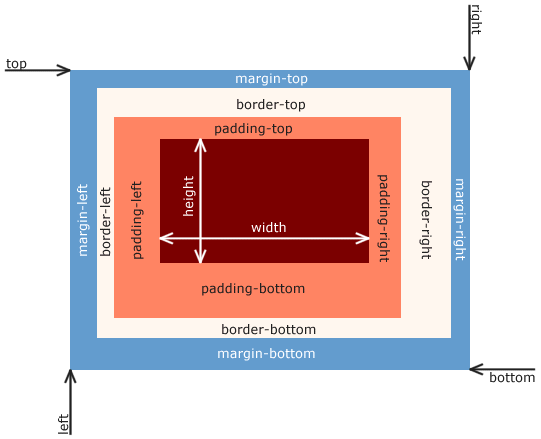
\includegraphics[width=0.8\linewidth]{abb/css_boxmodell}
  \caption[CSS-Boxmodell]{CSS-Boxmodell\cite{WikiCSS2014}}
  \label{fig:cssboxmodell}
\end{figure}	
	
\subsubsection{Spezifische Stylesheets} \glqq Dank der Mechanismen in CSS und HTML [... lassen sich] beliebige Stylesheets auf bestimmte Medien beschränken. In HTML-basierten Stylesheets geschieht dies mit Hilfe des Attributs \texttt{media} und gilt sowohl für \texttt{link}- wie auch \texttt{style}-Elemente. Das Attribut \texttt{media} akzeptiert entweder die Angabe eines einzelnen Mediums oder eine durch Komma getrennte Liste von Werten.\grqq{}\cite[S.434ff]{MeyeCasc2005} Die Angaben in Listing \ref{lst:css3media} bewirken eine gesonderte Formatierung für ein \texttt{print} Medium.

\vspace{1em}
\begin{lstlisting}[language=HTML5, caption=CSS3 medienspezifisches Stylesheet, label=lst:css3media]
<link rel="stylesheet" type="text/css" media="print" href="print.css">
\end{lstlisting}
	
Ein vorhandenes Stylesheet ohne Medieninformationen gilt für alle Medien. Ferner lassen sich die Medien auch näher beschreiben innerhalb des Stylesheets durch den \texttt{@media}-Block. Diesen \texttt{@media}-Blöcken können, neben den Medientypen, auch noch weitere Bedingungen hinzugefügt werden. In Listing \ref{lst:css3mediaquery} wird das Element mit der ID \texttt{inhalt} auf eine Breite von \texttt{800px} festgelegt. Ist das verwendete Ausgabemedium jedoch ein Bildschirm und hat nur eine Gesamtbreite von \texttt{1024px} wird das Element mit der ID \texttt{inhalt} auf eine Breite von nur noch \texttt{600px} und das \texttt{aside}-Element gar nicht mehr angezeigt.

\vspace{1em}
\begin{lstlisting}[language=CSS, caption=CSS3 eigenschaftsspezifisches Stylesheet, label=lst:css3mediaquery]
#inhalt {
	width: 800px;
}
 
@media screen and (max-width: 1024px) {
	#inhalt {
		width: 600px;
	}
	aside {
		display: none;
	}
}
\end{lstlisting}

\subsection{JavaScript}
Dieses Kapitel soll ein grundlegendes Verständnis für die Skriptsprache JavaScript aufbauen. Beginnend mit der Historie, Sandbox-Prinzip, hin zur Objektorientierung und den Sprachelementen, werden außerdem die einzelnen Datentypen, Werte und Variablen beschrieben. Im Detail werden dann die Operatoren, Schleifen und Kontrollstrukturen erörtert und durch Listings verdeutlicht. Des Weiteren ist das Document-Object-Model, die Ereignisverarbeitung und die asynchrone Kommunikation wichtig zum Verständnis des Frameworks jQuery, auf welchem letztendlich auch das SAP UI5-Framework basiert.

\subsubsection{Historie} JavaScript wurde 1995 von Netscape entwickelt, lizenziert und eingeführt. Um der Sprache von Anfang an einen Standardcharakter zu geben, wurde die Organisation \textit{European Computer Manufacturers Association} (ECMA) hinzugezogen. Unter dem Namen ECMAScript veröffentlichte die ECMA einen Industriestandard der JavaScript Sprache, der auf Netscapes JavaScript Spezifikation basiert. Da JavaScript eine proprietäre Sprache von Netscape ist, hat Microsoft seine eigene Variante, mit dem Namen JScript, veröffentlicht. JScript implementiert JavaScript vollständig, besitzt allerdings auch noch Zusatzfunktionen, wie z.B. Zugriff auf das Dateisystem und das Betriebssystem Windows. Mit Version 1.5 von JavaScript erhielt das DOM Einzug in die Implementierung. Da jeder Browser seinen eigenen JavaScript-Interpreter besaß, war es kaum möglich, einen einheitlichen Code für alle Browser zu entwickeln. Es musste auf alle Eventualitäten geachtet werden. Um diesem Missstand entgegenzuwirken, wurde das W3C hinzugezogen, um einen einheitlichen Sprachstandard zu etablieren. Jedoch entwickelte das W3C keinen konkreten JavaScript-Standard, sondern eine Schnittstelle - das erwähnte DOM. Die aktuelle JavaScript Version von 2010 ist 1.8.5 und ECMAScript liegt in Version 5.1 seit Juni 2011 vor. (vgl. \cite{SelfHtml20146})

\subsubsection{Sandbox-Prinzip} JavaScript wird innerhalb eines Browser in einer sogenannten Sandbox ausgeführt. Das bedeutet, es liegt in einem abgesichertem Speicherbereich, aus welchem es keinen Zugriff auf Objekte außerhalb des Browsern hat. Eine Ausnahme ist der Lesezugriff auf Dateien, die mittels des \texttt{input}-Elements von einem Nutzer selbst hoch geladen werden. Des Weiteren kann mit JavaScript auch nicht ohne weiteres auf bestimmte sicherheitskritische Funktionen des ausführenden Browser zugegriffen werden. Um beispielsweise das Browserfenster zu schließen, Symbolleisten ein- und auszublenden oder Zugriff auf die Seitenhistorie zu erlangen sind Nutzereingaben nötig. (vgl. \cite{WikiJS2014})

\subsubsection{Paradigma} \glqq JavaScript gehört zu den sogenannten objektorientierten Programmiersprachen (oder, um genauer zu sein, zu den objektbasierten Sprachen). Das Konzept der objektorientierten Programmierung (OOP) wird im Folgenden sehr stark vereinfacht erklärt.[...] In JavaScript ist (mit Ausnahme der Variablen) alles, worauf man zugreift, ein Objekt. Ein Objekt ist der Versuch, die reale Welt in eine Programmiersprachenumgebung abzubilden. Ein Standardbeispiel für Objekte ist etwa ein Auto. Das Auto an sich (als abstrakter Begriff) kann als Objekt angesehen werden, ein einzelnes Auto wird als Instanz des Objekts Auto bezeichnet.\grqq{}\cite[S.93]{WenzJava2008} Ein Auto bzw. ein Objekt lässt sich durch Parameter näher beschreiben. Diese Parameter gibt es in zwei Ausführungen, die Eigenschaften und Methoden. Bei einer Eigenschaft handelt es sich im Grunde um eine Variable die einen festen Bezug zum Objekt besitzt. Eigenschaften können gelesen und gesetzt werden. Ein Auto hat beispielsweise als Eigenschaft die Anzahl der Türen oder die Motorleistung. Methoden müssen hingegen nicht immer einen Informationswert zurückgeben. Bei dem Objekt Auto könnte es eine Methode \texttt{tunen()} geben die dann Einfluss auf die Eigenschaft Motorleistung nimmt.\par Im Kontext der Webentwicklung mit JavaScript existieren einige feste Objekte die zu jeder Zeit zur Verfügung stehen. Da wäre zum einen das \texttt{window}-Objekt, dass das aktuelle Browserfenster repräsentiert. Über die Eigenschaften und Methoden lassen sich Informationen zum Browserfenster erhalten und beispielsweise neue Fenster öffnen. Das \texttt{document}-Objekt bildet den Inhalt eines Browserfensters ab und stellt das Ausgangsobjekt für das DOM dar. Es steht in der Hierarchie direkt unter dem \texttt{window}-Objekt. Neben diesen Objekten existieren noch weitere, um den Browserkontext möglichst genau innerhalb einer JavaScript Anwendung verfügbar zu machen.(vgl. \cite{SelfHtml20147})

\subsubsection{Sprachelemente} JavaScript wird mit dem Unicode Zeichensatz geschrieben. Die 16-Bit-Codierung bei Unicode enthält fast sämtliche Zeichen der Schriftsprachen der Welt. Die Nutzung von Unicode trägt wesentlich zu der Internationalisierung bei. Bei der Groß- und Kleinschreibung unterscheidet JavaScript eindeutig. So müssen alle Schlüsselwörter und Bezeichner immer in der selben vorgegebenen Schreibweise geschrieben werden, damit sie vom JavaScript-Interpreter korrekt behandelt werden. Whitespace, Tabulatoren und Zeilentrenner werden vom Interpreter komplett ignoriert und können deshalb zur visuellen Strukturierung des Programmcodes genutzt werden. Dadurch kann der Programmcode leicht leserlich und verständlich formatiert werden, ohne dass dadurch die Logik verletzt wird. Das aus anderen Programmiersprachen bekannte Semikolon am Ende einer Anweisung ist in JavaScript nicht zwingend erforderlich. Eine Anweisung ist im Normalfall mit dem Ende der Zeile abgeschlossen. So muss ein Semikolon lediglich gesetzt werden, wenn sich mehr als eine Anweisung in der Zeile befinden oder eine Anweisung über mehrere Zeilen hinweg formuliert wurde. Fehlende Semikola werden vom Interpreter selbst gesetzt, was in bestimmten Fällen aber zum Bruch der Logik führen kann, wie in Listing \ref{lst:jssemikolon} zu sehen.(vgl. \cite[S.15ff]{FlanJava2007})

\vspace{1em}
\begin{lstlisting}[language=JavaScript, caption=JavaScript Logikbruch Semikolon, label=lst:jssemikolon]
// kein Interpretierungsfehler
a = 3
b = 4;

// korrekte Schreibweise in einer Zeile
a = 3; b = 4;

// Interpreter setzt Semikolon automatisch
return
true;
// falsche Interpretation anschliessend
return;
true;
\end{lstlisting}

Des weiteren gibt es einige Literale in JavaScript. \glqq Ein Literal ist ein Datenwert, der direkt in einem Programm vorkommt. Literale können zum Beispiel folgendermaßen aussehen:\grqq{}\cite[S.18]{FlanJava2007}

\vspace{1em}
\begin{lstlisting}[language=JavaScript, caption=JavaScript Literale, label=lst:jsliterale]
12                // Die Zahl zwoelf
1.2               // Die Zahl eins komma zwei
"Hallo Welt"      // Ein Text-String
'Hi'              // Noch ein String
true              // Ein Boolescher Wert
false             // Der andere Boolesche Wert
null              // Kein Objekt vorhanden
\end{lstlisting}
	
Im offiziellen Standard ECMAScript existieren außerdem Literale, die zur Initialisierung von Arrays und Objekten dienen. Neben den genannten Sprachelementen gibt es noch die Bezeichner. Ein Bezeichner ist ein Name in JavaScript. Er dient dazu Variablen, Funktionen und einige Schleifen-Marker zu benennen. Ein Bezeichner unterliegt gewissen Regeln. Zum einen muss das erste Zeichen ein Buchstabe, ein Unterstrich (\_) oder ein Dollar-Zeichen (\$) sein. Der restliche Bezeichner darf aus Buchstaben, Ziffern, Unterstrichen oder Dollar-Zeichen bestehen. Eine weitere Regel legt fest, dass ein Bezeichner nicht wie ein Schlüsselwort heißen darf. Tabelle \ref{tab:jskeywords} listet die Schlüsselwörter von JavaScript auf.(vgl. \cite[S.19]{FlanJava2007})

\vspace{1em}
\begin{center}
  \begin{tabular}{ | l | l | l | l | l | }
  \hline
  break & do & if & switch & typeof\\
  \hline
  case & else & in & this & var\\
  \hline
  catch & false & instanceof & thorw & void\\
  \hline
  continue & finally & new & true & while\\
  \hline
  default & for & null & try & with\\
  \hline
  delete & function & return & &\\
  \hline
  \end{tabular}
  \captionof{table}{JavaScript Schlüsselwörter}
  \label{tab:jskeywords}
\end{center}

\subsubsection{Datentypen und Werte} Werte, zur Berechnung, werden in Variablen mit bestimmten Datentypen gesichert. Dazu unterstützt JavaScript einige primitive Datentypen wie Zahlen, Text und boolesche Werte. Außerdem gibt es einen zusammengesetzten Datentypen, das Objekt, mit dem eine Sammlung von verschiedenen Werten dargestellt wird. So kann ein Objekt beispielsweise auch weitere Objekte beinhalten. Sind die Werte in geordneter nummerierter Reihenfolge, nennt man das Objekt Array. Integer ist der einfachste Datentyp. Mit ihm werden Zahlen dargestellt, egal ob ganze Zahlen oder Gleitkommazahlen. JavaScript behandelt jede Zahl als Gleitkommazahl und stellt diese im 64-Bit-Gleitkommaformat nach IEEE 754 dar. Integer-Literale werden in JavaScript als eine Folge von Ziffern geschrieben. Mit diesem Zahlenformat lassen sich alle ganzen Zahlen von einschließlich -2$^5$$^3$ bis 2$^5$$^3$ darstellen. Ein Hexadezimal-Literal wird mit einem \texttt{0x} oder \texttt{0X} begonnen gefolgt von einer Hexadezimalzahl. Bei Gleitkomma-Literalen wird der ganzzahlige Teil durch einen Punkt vom Bruchteil der Zahl getrennt. Des Weiteren können sie in der Exponentenschreibweise geschrieben werden. Um Text darzustellen, wird der Datentyp String verwendet. Ein String ist eine Folge von Unicode-Zeichen in einzelnen oder doppelten Anführungszeichen. Damit spezielle Zeichen innerhalb von Strings benutzt werden können, gibt es eine \textit{Escape-Sequenz} in Form eines Backslash (\textbackslash). So lassen sich Tabulatoren oder Zeilenumbrüche in einem String darstellen. Daneben gibt es die beiden booleschen Werte \texttt{true} und \texttt{false}. Sie werden zumeist bei Vergleichen als Wahrheitswert verwendet. Funktionen sind ein besonderer Datentyp. Denn diese Funktionen sind ein ausführbarer Programmcode. Sie werden einmal geschrieben und können dann beliebig oft benutzt werden. Einer Funktion lassen sich Argumente und Parameter übergeben, die dann in der Berechnung zur Verwendung kommen. Eine Funktion wird durch das Schlüsselwort \texttt{function} eingeleitet, gefolgt von einem optionalen Bezeichner und einer, durch Kommata, getrennten Liste von Argumenten und Parametern, die in runden Klammern eingeschlossen ist. Dann gibt es noch die Objekte, die eine Sammlung von nicht nummerierten Eigenschaften darstellen. Um auf eine Eigenschaft eines Objekts zuzugreifen, wird an den Objektbezeichner ein Punkt angehangen und dann der Name der Eigenschaft. Im Gegensatz dazu, kann auf die Eigenschaften eines Arrays nur über den Index zugegriffen werden. Das Schlüsselwort \texttt{null} ist ein spezieller Wert. Er steht für \textit{kein Wert} und wird häufig bei der Überprüfung von Variablen und Objekten verwendet.(vgl. \cite[S.22ff]{FlanJava2007})
	
\subsubsection{Variablen} \glqq Eine Variable ist ein Name, der mit einem Wert verbunden ist. Man spricht davon, dass die Variable den Wert speichert oder enthält. Variablen ermöglichen es [...], Daten in [...] Programmen zu speichern und zu bearbeiten.\grqq{}\cite[S.51]{FlanJava2007} Ein grundlegender Unterschied von JavaScript zu anderen Programmiersprachen besteht darin, dass Variablen nicht typisiert werden müssen. So kann einer JavaScript-Variable ohne Weiteres erst ein Zahlenwert und später eine Zeichenkette zugewiesen werden. Diese Art von Typisierung nennt man dynamische Typisierung(Loose Typing), da erst zur Laufzeit der tatsächliche Datentyp der Variablen feststeht. In anderen stark typisierten Sprachen wie C oder Java sind solche Konstrukte nicht zulässig, da einer Variable auch nur ein Wert, der ihrem Datentyp entspricht, zugewiesen werden kann. Eine Variable wird in JavaScript mit dem Schlüsselwort \texttt{var} und einem Bezeichner deklariert. Das Schlüsselwort \texttt{var} kann auch weggelassen werden, dann wird es vom Interpreter implizit gesetzt. Auf diese Weise deklarierte Variablen werden automatisch als globale Variabel deklariert. Soll eine Variable jedoch nur innerhalb eines Funktionsblocks Gültigkeit haben, ist die Verwendung des Schlüsselworts \texttt{var} unerlässlich. Aus diesem Grund sollte das Schlüsselwort immer zur Deklaration von Variablen genutzt werden. Initialisiert werden Variablen durch die Zuweisung eines Wertes mittels des Zuweisungsoperator (=). Dies kann auch mit der Deklaration in einem Schritt zusammengefasst werden.(vgl. \cite[S.52ff]{FlanJava2007})

\subsubsection{Operatoren} \glqq Durch Operatoren wird eine gewisse Anzahl von Variablen miteinander kombiniert. Beispiele für Operatoren sind die Grundrechenarten. Durch den Plus-Operator werden zwei Zahlen miteinander kombiniert, und als Ergebnis erhält man die Summe dieser beiden Zahlen. Man unterscheidet - auch je nach Typ der beteiligten Variablen - verschiedene Arten von Operatoren.\grqq{}\cite[S.69]{WenzJava2008} Mit den arithmetischen Operatoren lassen sich numerische Variablen miteinander verknüpfen und berechnen. Durch die dynamische Typisierung sollte man stets sicher sein, dass die Operanden auch Zahlen Variablen sind und keine String Variablen. Zu den arithmetischen Operatoren gehören die Addition (\texttt{+}), Subtraktion (\texttt{-}), Multiplikation (\texttt{*}), Division (\texttt{/}), die Restwertberechnung Modulo (\texttt{\%}) sowie die Negation (\texttt{-}). Außerdem sind noch zwei Operatoren zur In- (\texttt{++}) und Dekrementation (\texttt{--}) vorhanden. Der Plus (\texttt{+}) Operator hat noch eine zusätzliche Funktion. Er kann, neben der arithmetischen Addition, auch zur Zeichenverkettung verwendet werden. Neben den arithmetischen Operatoren, stehen in JavaScript auch Operatoren zur Verarbeitung von booleschen Werten bereit. Mit ihnen lassen sich Wahrheitswerte verknüpfen und vergleichen. Mit dem logischen UND (\texttt{\&\&}) beispielsweise wird ein boolescher Ausdruck darauf geprüft, ob beide Operanden als Wert \texttt{true} liefern. Ist dies der Fall, wird der Wert \texttt{true} für den booleschen Ausdruck zurück gegeben, ansonsten der Wert \texttt{false}. Das logische ODER (\texttt{||}) prüft einen booleschen Ausdruck im Grunde genauso wie ein logisches UND (\texttt{\&\&}) mit der Abweichung, dass bei einem logischen ODER (\texttt{||}) auch der Wert \texttt{true} für den gesamten booleschen Ausdruck zurück geliefert wird sollte nur der erste Operand den Wert \texttt{true} haben. Weiter gibt es boolesche Vergleichsoperatoren die bei Zahlenwerten aber auch mit Strings verwendet werden können. Zu ihnen gehören der Gleichheitsoperator (\texttt{==}), Ungleich (\texttt{!=}), Größer als (\texttt{\textgreater}), Kleiner als (\texttt{\textless}) und zuletzt Größer gleich (\texttt{\textgreater=}) und Kleiner gleich (\texttt{\textless=}).(vgl. \cite[S.71ff]{WenzJava2008})

\subsubsection{Schleifen} Um eine Anweisung innerhalb von JavaScript mehrfach ausführen zu lassen, bietet JavaScript Schleifenkonstrukte an. Darunter zählen die For-Schleife, die Do-While-Schleife und die While-Schleife. Jede Schleifenart hat in bestimmten Situationen Vor- und Nachteile gegenüber den anderen beiden Arten.\par Eine For-Schleife wird mit einem Startwert initialisiert und enthält außerdem eine Abbruchbedingung, sowie eine Befehlsfolge, die nach jedem Schleifendurchlauf ausgeführt wird. Listing \ref{lst:jssyntaxfor} zeigt die Syntax einer For-Schleife. Der Startwert ist auch die sogenannte Zählervariable, welche mit jedem Durchlauf durch die Befehlsfolge verändert wird. Die Abbruchbedingung überprüft diese Zählervariable und beendet die Schleife sollte die Bedingung nicht mehr zutreffen. Eine For-Schleife akzeptiert auch mehr als einen Startwert, welche durch Kommata voneinander getrennt werden.(vgl. \cite[S.75f]{WenzJava2008})

\vspace{1em}
\begin{lstlisting}[language=JavaScript, caption=Syntax For-Schleife, label=lst:jssyntaxfor]
for (Startwert; Abbruchbedingung; Befehlsfolge) {
  //Anweisung
}
\end{lstlisting}
	
For-Schleifen eignen sich vor allem, wenn man im Vorfeld weiß, wie oft die Anweisung wiederholt werden muss. Ist das nicht der Fall bietet sich die Do-While-Schleife an. Diese Art der Schleifen führt eine Anweisung mindestens einmal aus und überprüft dann zum ersten mal die Abbruchbedingung. Listing \ref{lst:jssyntaxdowhile} zeigt die Syntax einer Do-While-Schleife.

\vspace{1em}
\begin{lstlisting}[language=JavaScript, caption=Syntax Do-While-Schleife, label=lst:jssyntaxdowhile]
do {
  //Anweisung
} while (Abbruchbedingung);
\end{lstlisting}

In einigen Fällen kann die definitive Ausführung einer Anweisung, vor der ersten Überprüfung der Bedingung, nicht gewünscht sein. Dann sollte eine While-Schleife verwendet werden. Sie ist fast identisch der Do-While-Schleife. Der Unterschied besteht darin, dass die Abbruchbedingung als erstes überprüft wird und dann, sollte die Bedingung zutreffen, die Anweisung ausgeführt wird. So kann verhindert werden, dass die Anweisung fälschlicherweise ausgeführt wird, obwohl bestimmte Zuweisungen oder Funktionsaufrufe noch nicht durchgeführt wurden. Das Listing \ref{lst:jssyntaxwhile} zeigt die Syntax der While-Schleife.

\vspace{1em}
\begin{lstlisting}[language=JavaScript, caption=Syntax While-Schleife, label=lst:jssyntaxwhile]
while (Abbruchbedingung) {
  //Anweisung
}
\end{lstlisting}
	
Für den Fall, dass der aktuelle Schleifendurchgang oder die gesamte Schleife vorzeitig beendet werden soll, gibt es die beiden Schlüsselwörter \texttt{break} und \texttt{continue}. Die \texttt{break} Anweisung bewirkt, dass die gesamte Schleife beendet und das Programm nach der Schleife fortgeführt wird. Möchte man jedoch nur den aktuellen Schleifendurchgang beenden ist die \texttt{continue} Anweisung das Mittel der Wahl. Beide Anweisungen sind nur innerhalb von Schleifen gültig und erzeugen außerhalb dieser einen Syntaxfehler.(vgl. \cite[S.103f]{FlanJava2007})

\subsubsection{Kontrollstrukturen} Um den Programmablauf anhand von Fallunterscheidungen steuern zu können, sind von JavaScript die \texttt{if}-Anweisungen vorgesehen. Listing \ref{lst:jssyntaxifelse} zeigt die Syntax einer \texttt{if-else}-Anweisung. Ist die Bedingung wahr wird die Anweisung ausgeführt. Sofern eine \texttt{else} Anweisung vorhanden ist - sie ist optional - wird die darauf folgende Anweisung ausgeführt.(vgl. \cite[S.80]{WenzJava2008})

\vspace{1em}
\begin{lstlisting}[language=JavaScript, caption=Syntax If-else-Anweisung, label=lst:jssyntaxifelse]
if (Bedingung) {
  //Anweisung
} else {
  //Anweisung
}
\end{lstlisting}
	
Um den Programmcode übersichtlich zu halten, existiert noch eine \texttt{switch} Anweisung, die als eine Art Zusammenfassung für mehrere \texttt{if} Anweisungen zu verstehen ist. Listing \ref{lst:jssyntaxswitch} beschreibt die Syntax einer \texttt{switch} Anweisung. Zu beachten ist, dass in einer \texttt{switch} Anweisung eine \texttt{break} Anweisung als Abbruchbedingung unabdingbar ist. Lässt man sie weg, würde nach Ausführung der Anweisung des zuständigen \texttt{case} Blocks eventuell direkt der nächste passende \texttt{case} Block mindestens aber der \texttt{default} Block der \texttt{switch} Anweisung ausgeführt werden.

\vspace{1em}
\begin{lstlisting}[language=JavaScript, caption=Syntax Switch-Anweisung, label=lst:jssyntaxswitch]
switch (Ausdruck) {
  case Wert1:
    //Anweisung
    break;
  case WertN:
    //Anweisung
    break;
  default:
    //Anweisung
}
\end{lstlisting}

\subsubsection{Einbindung} Um ein, in JavaScript geschriebenes, Skript innerhalb eines HTML-Dokuments verwenden zu können, muss es erst einmal in dieses eingebunden werden. Eine Möglichkeit ist es, das Skript als separate Datei in das \texttt{head}-Element des HTML-Dokuments einzubinden. Listing \ref{lst:jseinbindunghead} zeigt das \texttt{script}-Element mit dem \texttt{src}-Attribut. Dieses Attribut verweist auf das externe Skript.

\vspace{1em}
\begin{lstlisting}[language=HTML5, caption=JavaScript Einbindung als separate Datei im \texttt{head}-Element, label=lst:jseinbindunghead]
<script src="script.js" type="text/javascript"></script>
\end{lstlisting}

Die andere Möglichkeit besteht darin, ein Skript direkt in das HTML-Dokument zu schreiben und mit einem \texttt{script}-Element zu umschließen. Dies muss auch nicht zwingend im \texttt{head}-Element passieren, sondern kann auch an anderer Stelle im Dokument sein. Dies ist je nach Anwendungsfall unterschiedlich. Listing \ref{lst:jseinbindungscript} zeigt diese Möglichkeit.(vgl. \cite[S.47]{AntoEinf2014})

\vspace{1em}
\begin{lstlisting}[language=HTML5, caption=JavaScript Einbindung in \texttt{script}-Element, label=lst:jseinbindungscript]
<script type="text/javascript"></script>
\end{lstlisting}

\subsubsection{Document Object Model} Das DOM ist eine Schnittstelle, um mit Skriptsprachen auf die Struktur eines HTML-Dokuments Einfluss nehmen zu können. Spezifiziert wurde das DOM vom W3C, um eine einheitliche Funktionsweise zu ermöglichen. Das DOM ist wie ein umgedrehter Baum aufgebaut. Jedes HTML-Element und auch Texte, die nicht von HTML-Elementen umschlossen sind, werden im DOM als Knoten (engl. node) dargestellt. HTML-Elemente, die innerhalb eines anderen HTML-Elements liegen, werden im DOM als Kindknoten (engl. child nodes) eingegliedert. Dadurch ist im DOM auch eine klare Hierarchie gegeben.(vgl. \cite[S.350]{WenzJava2008})\par Jeder Knoten im DOM beinhaltet zum einen Informationen über sich selbst und zum anderen Informationen über seinen Elternknoten und seine Kinderknoten. JavaScript hat dafür eigene Eigenschaften je Knoten definiert, mit denen auf diese Informationen zugegriffen werden kann. Mit den Eigenschaften \texttt{firstChild} und \texttt{lastChild} erhält man eine Referenz auf den ersten bzw. letzten Kindknoten des aktuellen Knotens. \texttt{nextSibling} und \texttt{previousSibling} liefern eine Referenz auf den nächsten bzw. vorherigen Kindknoten. \texttt{parentNode} ermöglicht den Zugriff auf den Elternknoten. Die beiden Eigenschaften \texttt{nodeName} und \texttt{nodeType} sind zur Bestimmung des Knoten selbst zuständig.

\vspace{1em}
\begin{lstlisting}[language=HTML5, caption=DOM5 Beispiel Definition, label=lst:html5beispieltable]
<table>
  <thead>
    <tr>
      <th>Produkt</th>
      <th>Preis</th>
    </tr>
  </thead>
  <tbody>
    <tr>
      <td>XYZ</td>
      <td>50,00</td>
    </tr>
  </tbody>
</table>
\end{lstlisting}

Listing \ref{lst:html5beispieltable} zeigt eine in HTML implementierte, Tabelle die in das entsprechende DOM umgewandelt wird, welches in Abbildung \ref{fig:dombeispielbaum} zu sehen ist.

\vspace{1em}
\begin{figure}[htb]
  \centering
  
\includegraphics[width=0.5\textwidth]{abb/dom_sampletree}
  \caption[DOM Beispielbaum aus Listing \ref{lst:html5beispieltable}]{DOM Beispielbaum aus Listing \ref{lst:html5beispieltable}}
  \label{fig:dombeispielbaum}
\end{figure}

Selbstverständlich bietet das DOM die Möglichkeit der Modifizierung. So lassen sich Knoten nicht nur ändern, sondern auch entfernen und neu hinzufügen. Aufgrund der Baumstruktur ist es möglich einen Knoten zu löschen, ohne die Integrität des Baumes zu zerstören.

\subsubsection{Ereignisse} Interaktive JavaScript Applikationen kommunizieren mit dem Browser über Events. Der Browser erzeugt für eine Vielzahl von Nutzeraktionen Events, welche dann wiederum im Applikationscode abgefangen und verarbeitet werden können. In der DOM0 Spezifikation werden Events lediglich an die Elemente verteilt, an denen sie auftreten. Ist an diesem Element dann ein Event-Listener registriert, wird dieser ausgeführt. DOM2 hat die sogenannte Event-Propagation eingeführt. Diese Eventverteilung ist in drei Phasen aufgeteilt. Als erstes steht das Abfangen. Dabei werden Events vom \texttt{document}-Objekt den Dokumentbaum hinunter gereicht, bis sie am Zielelement angelangt sind. Besitzt ein Vorgängerelement im Dokumentbaum allerdings einen abfangenden Event-Listener wird auch dieser ausgelöst. Als nächstes löst das Event den Listener am Zielelement aus, was der DOM-Level-0 Spezifikation gleicht. Die dritte Phase ist das sogenannte \textit{bubbling}. Hierbei steigt das Event wie ein Bläschen in der Dokumentenhierarchie zum \texttt{document}-Objekt auf. Das Aufsteigen eines Events ist aber je nach Event unterschiedlich. Einige steigen auf, andere nicht. Ein Event mit dem ein Formular beispielsweise abgeschickt wird, muss nicht weiter im Dokumentbaum nach oben propagiert werden. Mausklick-Events hingegen können für das gesamte Dokument sinnvoll verarbeitet werden und werden daher immer im Dokument aufsteigen.\par Ein Event-Listener kann auf drei unterschiedliche Arten an ein HTML-Element gebunden werden. Eine Möglichkeit ist den Event-Listener direkt an das HTML-Element mittels eines entsprechenden Event Attributs zu binden. So zu sehen in Zeile 1 in Listing \ref{lst:jseventhandler}. 

\vspace{1em}
\begin{lstlisting}[language=JavaScript, caption=JavaScript Event-Handler Beispiek, label=lst:jseventhandler]
<input type="button" name="b1" value="Drueck mich"
 onclick="alert('Button gedrueckt!');">

document.b1.onclick = function() { alert('Button gedrueckt!'); };

document.b1.addEventListener("click", click, false);
function click() { alert('Button gedrueckt!'); };
\end{lstlisting}

Da HTML statisch ist, ist auch der Event-Listener statisch. Komplexe Applikationen verlangen aber eine dynamische Bindung von Listenern. Aus diesem Grund wurden mit DOM2 zwei weitere Möglichkeiten, einen Event-Listener zu registrieren, standardisiert. So kann der Listener einerseits einfach einer Eigenschaft des DOM Objekts zugewiesen werden. Daraus resultiert ein klar strukturierter Code im HTML und JavaScript. Die Wartbarkeit wird außerdem verbessert. Andererseits lässt sich ein Listener über eine Objektmethode binden. Diese Methode erwartet drei Argumente. Das erste Argument bestimmt das Event, auf welches der Listener reagieren soll. Das zweite Argument ist die Funktion, die beim Eintreten des Events ausgeführt werden soll. Das dritte Argument, ein Boolescher Wert, legt fest ob der Event-Listener das Event nur abfängt wenn es direkt am Element oder dessen Kind Elementen auftritt. Dann muss dieser Wert \texttt{false} sein. Ansonsten kann der Event-Listener auch Events abfangen, die im Geltungsbereich ihm übergeordnet sind. Diese beiden Möglichkeit sind in Listing \ref{lst:jseventhandler} ab Zeile 4 zu sehen. Nachfolgend ist eine Übersicht einiger wichtiger Events.(vgl. \cite[S.428ff]{FlanJava2007})

\vspace{1em}
\begin{compactitem}
  \item onabort (bei Abbruch)
	\item onblur (beim Verlassen)
	\item onchange (bei erfolgter Änderung)
	\item onclick (beim Anklicken)
	\item ondblclick (bei doppeltem Anklicken)
	\item onerror (im Fehlerfall)
	\item onfocus (beim Aktivieren)
	\item onkeydown (bei gedrückter Taste)
	\item onkeypress (bei gedrückt gehaltener Taste)
	\item onkeyup (bei losgelassener Taste)
	\item onload (beim Laden einer Datei)
	\item onmousedown (bei gedrückter Maustaste)
	\item onmousemove (bei weiterbewegter Maus)
	\item onmouseout (beim Verlassen des Elements mit der Maus)
	\item onmouseover (beim Überfahren des Elements mit der Maus)
	\item onmouseup (bei losgelassener Maustaste)
	\item onreset (beim Zurücksetzen des Formulars)
	\item onselect (beim Selektieren von Text)
	\item onsubmit (beim Absenden des Formulars)
	\item onunload (beim Verlassen der Datei)
\end{compactitem}

\subsubsection{AJAX}
AJAX steht als Akronym für \textit{Asynchronous JavaScript and XML}. Geprägt wurde der Begriff AJAX von Jesse J. Garret.(vgl. \cite{JesseJGarret}) Es ist keine eigenständige Technologie, sondern vielmehr eine Bündelung einiger der verbreitetsten Web Technologien. Dazu gehört das Hypertext Transfer Protocol (HTTP), JavaScript, XML und neuerdings auch das JavaScript Object Notation (JSON) Format. Entwickelt wurde diese Technik von Microsoft, speziell von den Outlook Entwicklern. Diese benötigten eine Möglichkeit, um HTTP-Anfragen an einen Server abzusetzen, ohne ein permanentes Neuladen der kompletten Webseite zu verursachen, z.B. beim Prüfen ob neue Mails vorhanden sind. Diese Anfragen sollten im Hintergrund ausgewertet und der entsprechende Teil der Webseite durch JavaScript, mit den nachgeladenen Informationen, verändert werden. Dadurch muss der Anwender nicht mit seiner Dateneingabe warten bis der Server mit der Auswertung, der vorher eingegeben Daten, fertig ist.\par Technisch erfolgt dies in drei Schritten. Zuerst wird ein AJAX-Objekt erzeugt, dazu haben die Browser Hersteller das \texttt{XMLHttpRequest}-Objekt implementiert. Über dieses Objekt wird eine Verbindung zur Zielseite hergestellt. Als Parameter benötigt das Objekt die HTTP Übertragungsmethode, sprich \texttt{GET} oder \texttt{POST}. Außerdem benötigt das Objekt die URL der Zielseite und zuletzt einen Booleschen Wert, der das Skript entweder synchron oder asynchron ausführen lässt. Zuletzt wird eine Rückgabefunktion angegeben, die aufgerufen wird, sobald der Server mit der Verarbeitung fertig und seine Antwort auf der Client Seite angekommen ist.(vgl. \cite[S.392ff]{WenzJava2008}) Abbildung \ref{fig:ajax} zeigt schematisch die Kommunikation zwischen Client und Server mit der AJAX Technik. Bekanntestes Beispiel einer AJAX-Implementation ist der Vorschlag-Mechanismus der Google Suche.

\vspace{1em}
\begin{figure}[htb]
  \centering
  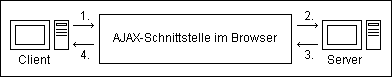
\includegraphics[width=1\textwidth]{abb/ajax_uml}
  \caption[AJAX Client/Server Kommunikation]{AJAX Client/Server Kommunikation \cite{ajax}}
  \label{fig:ajax}
\end{figure}

\subsubsection{jQuery}
jQuery ist die am meisten verbreitetste JavaScript Bibliothek im Internet. Mit 94,7\% Marktanteil (Stand 19.1.2015) ist jQuery klar der Marktführer der JavaScript Bibliotheken. Ganze 61,7\% der vom W3 Technology Survey analysierten Webseiten verwenden jQuery in ihrer Implementierung. (vgl. \cite{w3tech}) Die freie JavaScript Bibliothek jQuery stellt unter anderem umfangreiche Funktionen zur Manipulierung des DOM bereit. Daneben ist die Verwendung der AJAX Technik enorm vereinfacht worden. Animationen und Effekte lassen sich schnell und unkompliziert mit der Bibliothek realsieren. Wie aus CSS bekannt verwendet jQuery Selektoren, um auf die DOM Knoten zuzugreifen. Dank dem Programmierkonzept der \textit{fluent interfaces}, was soviel bedeutet wie sprechende Schnittstellen, kann ein erzeugtes jQuery Objekt sehr einfach an andere Funktionen weitergegeben werden.(vgl. \cite{wikijquery}) \glqq jQuery wird von \url{http://docs.jquery.com/} geladen und per Script-Tag in die HTML-Dokumente eingebunden.

\vspace{1em}
\begin{lstlisting}[language=HTML5, caption=jQuery Einbindung, label=lst:jqueryscript]
<script type="text/javascript"src="jquery.js"></script>
\end{lstlisting}

Die grundlegende Funktion von jQuery ist die Funktion \texttt{jQuery()} oder auch mit verringertem Schreibaufwand \texttt{\$()}, deren Verhalten abhängig ist von den jeweils gesetzten Parametern. Dabei fasst (sammelt) jede \texttt{\$()}-Funktion einen oder mehrere Knoten eines DOM-Baumes zusammen. In der einfachsten Form wird dann nur ein Ausdruck übergeben - meistens ein CSS-Selektor -, der alle passenden Elemente im Dokument findet.\grqq{}\cite{itwissenjquery}

\vspace{1em}
\begin{lstlisting}[language=JavaScript, caption=jQuery Selektor Syntax, label=lst:jqueryselektor]
$("selektor").funktionsname({ function({ }); });
\end{lstlisting}
	
Listing \ref{lst:jqueryselektor} zeigt die übliche Syntax einer jQuery-Anweisung. Über den Selektor werden die Funktionen des erzeugten Objekts aufgerufen und eine entsprechende Rückgabefunktion wird außerdem übergeben, um auf das Ergebnis der Objektfunktion reagieren zu können.

%\paragraph{Ereignisse}$\;$ \\
%// unterschiede zum JS Standard bei der Definierung, Einfachheit\\
%
%// Übersicht der wichtigsten Funktionen zu Events
%\vspace{1em}
%    \begin{compactitem}
%	    \item .bind – Handler an Event binden
%	    \item .on – Handler an Event binden
%	    \item .blur – Ereignis, wenn ein Element den Fokus verliert
%	    \item .click – Klick mit der Maustaste
%	    \item .dbclick – Doppelklick mit der Maustaste
%	    \item .hover – Mauszeiger bewegt sich über ein Element
%	    \item .mousemove – Mauszeiger bewegt sich in einem Element
%	    \item .keypress – eine Taste der Tastatur wird gedrückt
%	    \item .keyup – eine Taste der Tastatur wird losgelassen
%	    \item .change – ein Formularfeld wird verändert
%    \end{compactitem}
%    
%\paragraph{DOM-Manipulation}$\;$ \\
%// DOM Manipulation kurz anreißen\\

%\subsection{ABAP}
%// Herkunft/Entstehung\\
%// Grundlagen\\
%// Wichtige Elemente (OpenSQL)\\

\subsection{SAP UI5-Framework}
Kapitel 2.4 beschreibt das SAP UI5-Framework der SAP AG. Beginnend mit einem kurzen Exkurs über die aktuelle UI-Strategie der SAP AG, um zu erörtern wieso die SAP AG dieses Framework entwickelt hat. Im Anschluss folgt eine allgemeine Definition, sowie die Beschreibung der verwendeten Softwarearchitektur. Zuletzt folgt eine kurze Erklärung des OData-Protokolls und die Positionierung des Frameworks, innerhalb einer SAP NetWeaver Landschaft.

\subsubsection{SAP User Interface Strategie}
Die SAP AG definiert ihre momentane \textit{User Experience} (UX) Strategie durch den Styleguide SAP Fiori und drei Schlagwörter -- \textit{New}, \textit{Renew} und \textit{Enable}. Unter \textit{New} wird verstanden, dass Entwicklern und Kunden neue Tools zur Entwicklung von SAP Applikationen zur Verfügung gestellt werden. \textit{Renew} bedeutet, dass die vorhandenen Kernszenarien auf das neue UX portiert werden. SAP Screen Personas, auf das im Rahmen der Bachelorarbeit nicht weiter eingegangen wird, gehört zum Schlagwort \textit{Enable}. Kurz gesagt soll mit diesem Toolset das vorhandene UI der SAP Software an das Corporate Design eines Unternehmens angepasst werden können.(vgl. \cite{SAPUX})

\vspace{1em}
\begin{figure}[htb]
  \centering
  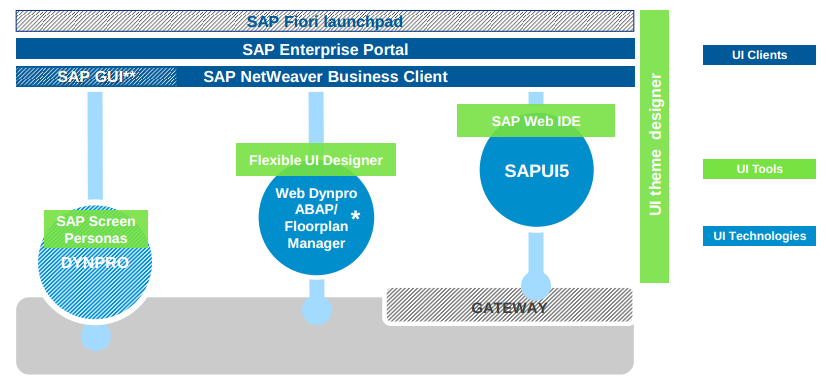
\includegraphics[width=0.9\textwidth]{abb/sap_key_ui_tools}
  \caption[SAP Schlüssel UI Tools und Technologien]{SAP Schlüssel UI Tools und Technologien \cite{SAPUXPDF}}
  \label{fig:sapkeyuitools}
\end{figure}

\subsubsection{Definition}
SAP UI5 ist ein \textit{Software Development Kit} (SDK) zur Entwicklung von Desktop- und mobilen Anwendungen die in einem Browser ausgeführt werden. Das Framework bündelt eine Vielzahl an Technologien und Bibliotheken, um den Entwicklungsprozess solcher Anwendungen bestmöglich zu unterstützen. Grundsätzlich basieren die, mit dem SDK entwickelten, Anwendungen auf den aktuellen Web Entwicklungsstandards, dazu gehören HTML5, CSS3 und JS. HTML5 und CSS3 werden dafür verwendet Struktur und Aussehen der Applikationen zu gestalten. Bei JS hat man sich außerdem dazu entschieden, zusätzlich die populäre Erweiterungsbibliothek jQuery zu nutzen.(vgl. \cite{BuiltWith2014}) Das komplette SAP UI5-SDK ist freie Software und kann ohne jegliche SAP-Lizenz bezogen und betrieben werden.

\subsubsection{Architektur}
\glqq Das Model-View-Controller [(MVC)] Architekturmuster strukturiert die Softwareentwicklung in die drei Einheiten: Datenmodell (Modell), Präsentation (View) und Steuerung (Controller). Durch diese Trennung können die einzelnen Komponenten leichter erweitert, ausgetauscht oder wiederverwendet werden. Abbildung [... \ref{fig:mvcarch}] zeigt dieses Architekturmuster.
	
\vspace{1em}
\begin{figure}[htb]
  \centering
  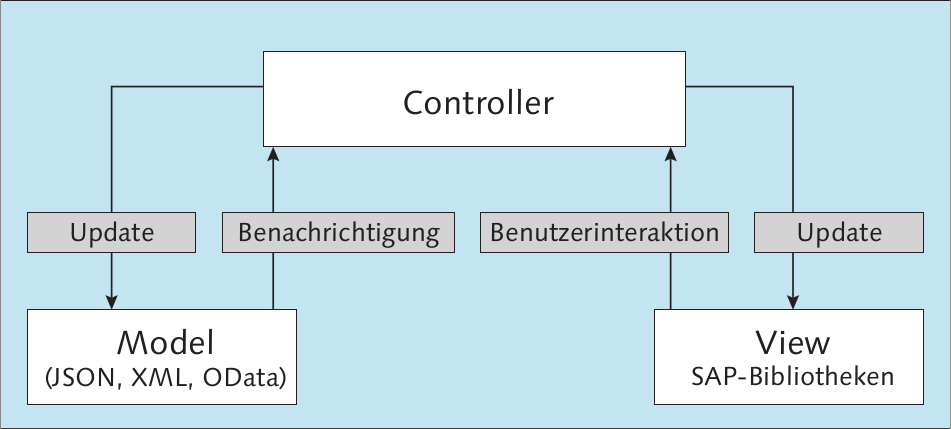
\includegraphics[width=0.75\linewidth]{abb/mvc_arch2}
  \caption[MVC-Architekturmuster]{MVC-Architekturmuster \cite[S.124]{AntoEinf2014}}
  \label{fig:mvcarch}
\end{figure}

Durch diese Trennung können z. B. zwei verschiedene Endgeräte das gleiche Modell verwenden; der View wird z. B. einmal für die Desktop-Anwendung und einmal für das mobile Endgerät implementiert.\grqq{}\cite[S.123]{AntoEinf2014}

\paragraph{Modell}$\;$ \\
Mit dem Modell wird das Datenmodell abgebildet. Neben dem Datenbankzugriffsmechanismus stellt es die Applikationsdaten bereit und kann zudem auch die dazugehörige Geschäftslogik enthalten.

\paragraph{View}$\;$ \\
Benutzeraktionen werden vom View erfasst und zur weiteren Verarbeitung an den Controller weitergegeben. Damit fungiert das View als Präsentationsschicht zur visuellen Darstellung auf den verschiedenen Endgeräten.

\paragraph{Controller}$\;$ \\
Der Controller ist die zentrale Steuereinheit. Er nimmt Benutzeraktionen vom View entgegen und verarbeitet diese weiter. Ein Controller kann mehrere Views verwalten, zu jedem View gehört mindestens ein Controller. Bei Datenänderungen durch den Anwender koordiniert der Controller die Kommunikation mit dem Modell.(vgl. \cite[S.123f]{AntoEinf2014})

\subsubsection{OData Protokoll}
\glqq Das \textit{Open Data Protocol} (OData) ist ein von Microsoft veröffentlichtes Protokoll. Das Protokoll basiert auf HTTP und baut auf den älteren Protokollen [Open Database Connectivity] (ODBC) und [Java Database Connectivity] (JDBC) auf. OData ist primär für die sogenannten CRUD-Operationen, (Create, Read, Update und Delete) implementiert worden.\grqq{}\cite[S.168]{AntoEinf2014} Von der SAP AG ist der Einsatz der SAP NetWeaver Gateway Software vorgesehen, um einen entsprechenden OData-Service im Backend bereitzustellen. Dadurch wird ein direkter Zugriff auf die dahinterliegenden Systeme verhindert. OData stellt eine API nach dem \textit{Representational State Transfer} (REST) Paradigma bereit. Ein REST-Service hat vier Eigenschaften die erfüllt sein müssen. Dazu gehört die Adressierbarkeit, jeder REST-Service hat eine eindeutige Adresse die URL (engl. Uniform Resource Locator). Der REST-Server muss die angeforderten Daten in unterschiedlichen Formaten zurückgeben können, wie zum Beispiel HTML, JSON oder XML. Zustandslosigkeit ist eine weitere Eigenschaft. Sie besagt, dass weder der Server, noch die Applikation, Zustandsinformationen zwischen zwei Nachrichten speichert. Jede Anfrage an den Server ist in sich abgeschlossen. Die letzte Eigenschaft beschreibt die Operationen, die ein REST Service bereitstellt. Bei einem Zugriff über HTTP werden die Methoden \texttt{GET}, \texttt{POST}, \texttt{PUT} und \texttt{DELETE} verwendet, um die CRUD Operationen zu ermöglichen.(vgl. \cite{wikirest})

\subsubsection{Positionierung im Netweaver Stack}
Eine mit SAP UI5 entwickelte Applikation wird als Business Server Page (BSP) Applikation auf dem SAP ABAP Application Server (AS) abgelegt. Von dort kann sie über die verschiedenen Endgeräte abgerufen werden. Aufgrund der verwendeten Technologien läuft die Anwendung weitestgehend auf dem jeweiligen Endgerät. Der ABAP AS dient lediglich dazu eingehende Anfragen, die vorher vom SAP NetWeaver Gateway entgegengenommen und weitergeleitet wurden, zu verarbeiten und eine entsprechende Antwort zurückzuschicken. Natürlich kann man auf das Gateway verzichten, was aus Sicherheitsgründen jedoch nicht zu empfehlen ist. Aufgrund des verwendeten OData Protokolls und der REST-Technik können problemlos Lastverteiler eingesetzt werden, wodurch eine einfache Möglichkeit zur Skalierung geboten wird.(vgl. \cite{SAPFIORIARCH}) Die Abbildung \ref{fig:sapui5arch} zeigt eine schematische SAP-Landschaft in der SAP UI5 integriert ist.

\vspace{1em}
\begin{figure}[htb]
  \centering
  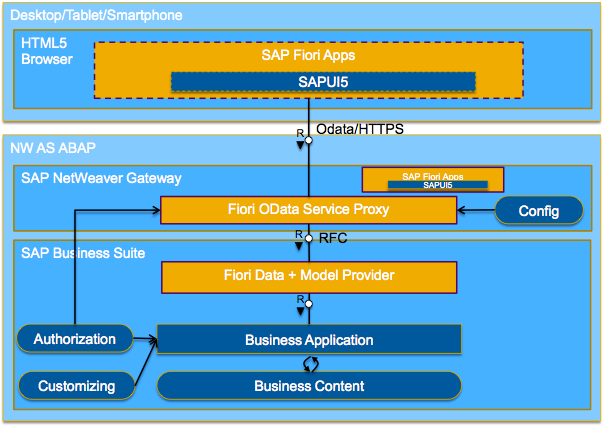
\includegraphics[width=0.8\linewidth]{abb/sap_ui5_architecture}
  \caption[Einordnung von SAP UI5 in die SAP-System-Landschaft]{Einordnung von SAP UI5 in die SAP-System-Landschaft \cite{SAPFIORIARCH}}
  \label{fig:sapui5arch}
\end{figure}